\documentclass[a4paper,UKenglish,cleveref,thm-restate]{lipics-v2021}
\usepackage{hyperref}
\usepackage{booktabs}
\usepackage{amsmath}
\nolinenumbers

\title{Range Minimum Queries}
\author{Henrik Iver Thorøe}{Karlsruhe Institute of Technology, Germany}{henrik.thoroe@student.kit.edu}{https://orcid.org/0009-0004-9517-1060}{}
\authorrunning{H. Thorøe}
\hideLIPIcs

\begin{document}
\maketitle


\section{Introduction}
The task submission contains:
\begin{itemize}
	\item The report and its source code under /report
	\item The plots under /plots
	\item The default input generator and build files with slight modifications
	\item The Rust source code under /rmq-rust
\end{itemize}

The source code itself is structured using the following components:
\begin{itemize}
	\item input.rs: Function to read the input data (as provided)
	\item main.rs: Entry point for benchmarking and to bootstrap all files 
	\item rmq.rs: The RMQ trait and module file for implementation re-export 
	\item rmq/<name>.rs: Implementations for the required data structures
	\item rmq/util.rs: A file for utility functions, containing a min\_of that is faster at getting the min element from a slice than the default iterator impl. 
\end{itemize}

\section{Methods}

\subsection{Naive}

An implementation that computes each query on the fly. No additional data structures are used, which results in 
a space overhead of $O(1)$. The queries are answered by simply returning the minimum of the 
(inclusive) range, which is computed in $O(n)$.

\subsection{Stored}

The 'CachedQuery' implementation pre-computes all possible queries and stores them in an additional 
array of size $O(n^2)$ words. To build the lookup table, the build function iterates over the data.
In each iteration a minimum is stored and updated in the nested loop, which iterates from the starting 
index to the end of the dataset. At each sub-iteration either the preceding minimum is stored, or, if the new 
element is smaller, the minimum is updated and stored. The build process finishes in $O(n^2)$. 

The lookup calculates the index of the result based on the range indicators and returns it in $O(1)$.

\subsection{Sparse Table}

The sparse table implementation stores the minimum for each sliding window of size $2^l$, 
where $l$ is in the range $[0, \lfloor\log_2{n}\rfloor]$. A query calculates the largest $l$,
so that the window of size $2^l$ fits into the difference of the range indicators. 
We can then take the first window starting in our sliding window and the last window ending 
in our range. The two windows cover the full range and the range minimum is therefore the 
minimum of the two sliding windows. 

The implementation has a space overhead of $O(n \log{n})$ words. It allocates an additional 
array of size $n\cdot\lfloor\log_2{n}\rfloor$ elements. Doing so wastes some space but stays 
inside the theoretical asymptotic boundaries, while making the data structure a little easier 
to understand. To build the sparse table, the original $n$ elements are copied to the start of
the new table array. The remaining levels are built iteratively. We utilize that in the previous level
two non-overlapping windows cover the same elements that our new window will cover. We therefore take 
for each new sliding window the minimum of the two matching windows in the previous level as our new 
minimum.

Queries can now be performed in $O(1)$. We perform the query as described in theory. The method 
calculates the level from the difference of the range indicators and can afterwards derive the 
exact indices for our sliding windows.  

\subsection{Segment Tree}

The segment tree stores a binary tree with the original data as leaves. Each parent node 
stores the minimum of the two child nodes. A query moves from the leaves up the tree until 
the common parent is found. Because the parent is always smaller than or equal to the child nodes,
the range minimum is found. As we move up the balanced binary tree a query takes $O(\log{n})$ time.
Storing the tree comes at an overhead of $O(n)$. 

For building the tree, we start by allocating an array of size $2n$. The original data is copied 
to the end of the array. While we have not reached the root node, we take the last level and 
$k$ preceding elements, where $k$ is the number of elements in the last created level. 
We then assign each of the elements in the current level the minimum of the two child elements in 
the lower level. 

The query is optimized to eliminate branching, which greatly improved performance in the 
benchmarks. First, $n$ is added to the range boundaries to move them to the positions of the leaf 
nodes in our tree array. Afterwards we iterate until the left boundary is greater than or equal to the right boundary, 
which means we reached the common parent. As described previously, at most $\log{n}$ iterations are performed. 
In each iteration we first create a mask that is 0 if the indices are odd and fully 1 otherwise. Using this mask 
we can update our result value only if the index is odd. To move to the next higher level we divide the indices by 2.
For our left index we need to consider that if it is odd, we need to move one horizontal index to the right before 
dividing by two. Otherwise we would move to the parent of the child, which would have the left child outside the 
range.  

\subsection{Block Sparse Table}

The block-based sparse table works similarly to the standard sparse table, but 
divides the data into blocks of fixed size, of which the minima are then stored in a 
sparse table. A reference to the original data allows us to answer queries that are not fully covered by the blocks. 

To build the data structure, we first compute the block minima. The array of the minima is then 
used to initialize a sparse table as introduced previously. The block implementation is therefore 
dependent on the sparse table implementation. As the sparse table takes $O(n\log{n})$ words of 
additional space our block-based approach takes $O(\frac{n}{s}\log{\frac{n}{s}})\equiv O(\frac{n}{s}\log{n})$ 
of additional words.

The query is performed by first calculating the block indices of the range indicators.
Those are then used to fetch the minimum value contained entirely in the blocks. 
If tails exist, the minimum is updated by iterating over those elements. 
The tails can have a maximum length of less than the block size, as they would otherwise
be contained in another block. We therefore get a query complexity of $O(1 + 2S) \equiv O(S)$.

\subsection{Block Sparse Table (Precomputed)}

The precomputed variant of the block-based sparse table works similarly to the previous implementation,
but during build time we create S suffix and prefix minima for each of the $\frac{N}{S}$ blocks, leading 
to an overhead of $O(2\cdot S\cdot\frac{N}{S})\equiv O(N)$ words.

The query differs in that we look up both the block minima and the suffix/prefix minima
from our tables. We therefore reduce query complexity to $O(1)$, as we do not need to iterate over the tails anymore.

\subsection{Cartesian Tree}

Cartesian trees are used to reduce space usage to linear, while maintaining constant query time.

The build process is similar to the block-based sparse table, but instead of storing the prefix/suffix
minima in a table, we store the shape of the Cartesian tree describing each block. 
We therefore need two additional arrays. The first array associates each block with a unique shape id. 
The second array stores the precomputed query results for each shape. During the build process
we use a hash map as a lookup table for each different tree signature. This avoids redundant computation 
of the query results, as they are equal for the same shape, regardless of the actual values. 

The query is performed by first calculating the leading and trailing block of the 
query. For the fully enclosed blocks, the sparse table is queried. We once again reuse the 
previous sparse table implementation here. The tails and heads in non fully enclosed 
blocks are queried by looking up the shape of the block and the local index of the query inside the 
given shape. The query results are finally combined to return the minimum. As each lookup (sparse table
and Cartesian trees) is constant, the full query is also constant.

\section{Results}

\subsection{Setup}

The benchmarks were run on a MacBook Pro with an M1 Pro chip. 
The compiler flags are as default, with the only change being 
link-time optimizations set to fat. Correctness has been verified 
by asserting the same sum for each n and implementation.

\subsection{Query Time Analysis}

The Naive and CachedQuery implementations are only benchmarked for up 
to $10^4$ elements. For the Naive implementation, compute time would 
be an issue for larger input sizes, while the CachedQuery would
use too much memory for the test system. As seen in \autoref{fig:query_time}, 
both implementations have a linear query time in the logarithmic plot.
This indicates different things for each. The naive implementation has a real 
linear query time, which is represented here. The CachedQuery on the other side 
has a theoretical query complexity of $O(1)$. The reason for the linear 
query time is likely due to the quadratic space usage, which leads to 
high numbers of cache misses. It is expected that the CachedQuery would increase 
roughly linearly until it settles at a constant query time, when 
each query has an amortized latency of a DRAM access. 

The two largest PrecomputeBlock implementations have their lowest latency at 
around $10^5$ elements. For lower input sizes, the query time is worse than that of 
other data structures, while for higher input sizes the query time is leading.
\autoref{sec:block_sizes} discusses possible reasons for this behaviour.

The SegmentTree implementation shows a slight linearly growing slope
which matches the expected logarithmic query complexity.

All other plots show the same general shape and mostly differ in absolute distance. 
We can see that for input sizes up to $10^6$ for Block and $10^4$ for the remaining
plots the query time stays constant per plot 
and bends upward afterwards. As they use different implementations, it is likely
that the bend is caused by a switch from 
compute bottleneck to a memory access bottleneck.

\begin{figure}[h]
	\centering
	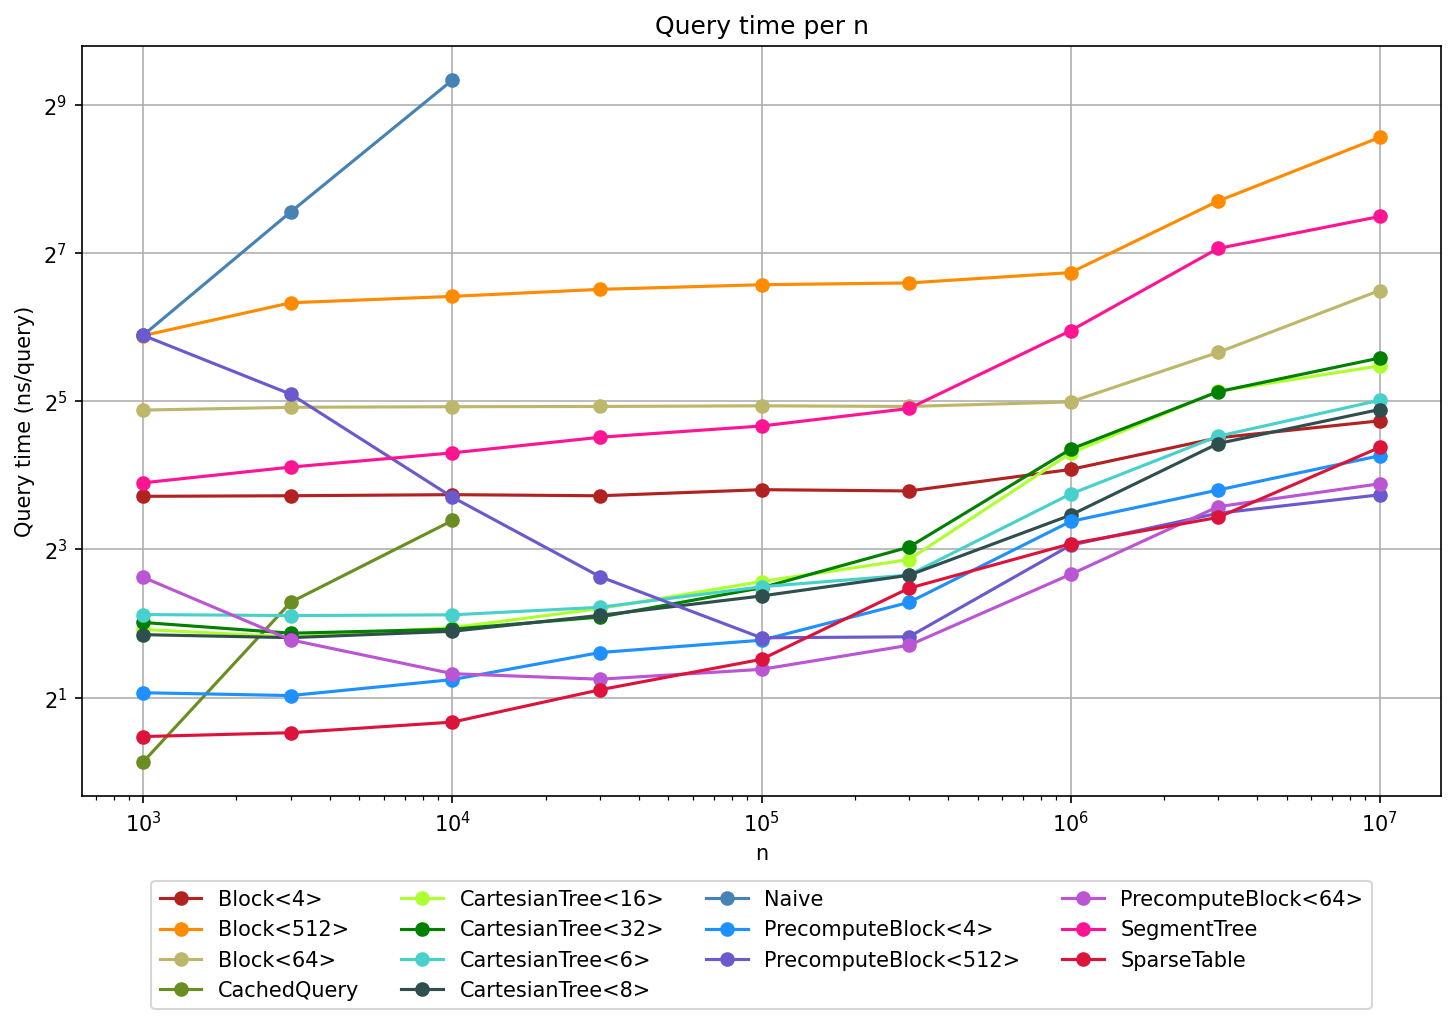
\includegraphics[width=.8\linewidth]{../plots/query_time.png}
	\caption{Query time per implementation for different input sizes.}
	\label{fig:query_time}
\end{figure}

\subsection{Space Analysis}

\autoref{fig:space} shows the space usage of each implementation. Both the 
x- and y-axis are logarithmic. The x-axis represents the number of elements 
and the y-axis the bits used per element. 

The Naive implementation uses a
constant amount of space, which is why the per element space usage falls 
linearly with $\frac{1}{n}$. The CachedQuery also behaves as expected for 
quadratic space usage.

SegmentTree and CartesianTree display a constant plot, as they use linear space.
The SparseTable and derived Block and PrecomputeBlock plots rise slowly
due to their additional logarithmic factor in space usage. 
The Block variants show a clear trend of lower space usage the larger the 
block size gets. 

An important comment for the Cartesian tree implementation is that 
for larger block sizes, their respective plots show clear deviation
from the expected linear space usage. This might be a result of 
choosing a block size significantly different from the theoretical 
optimal size of $s=\frac{1}{4}log_2(n)\approx2$ for $n=10^7$.

\begin{figure}[h]
	\centering
	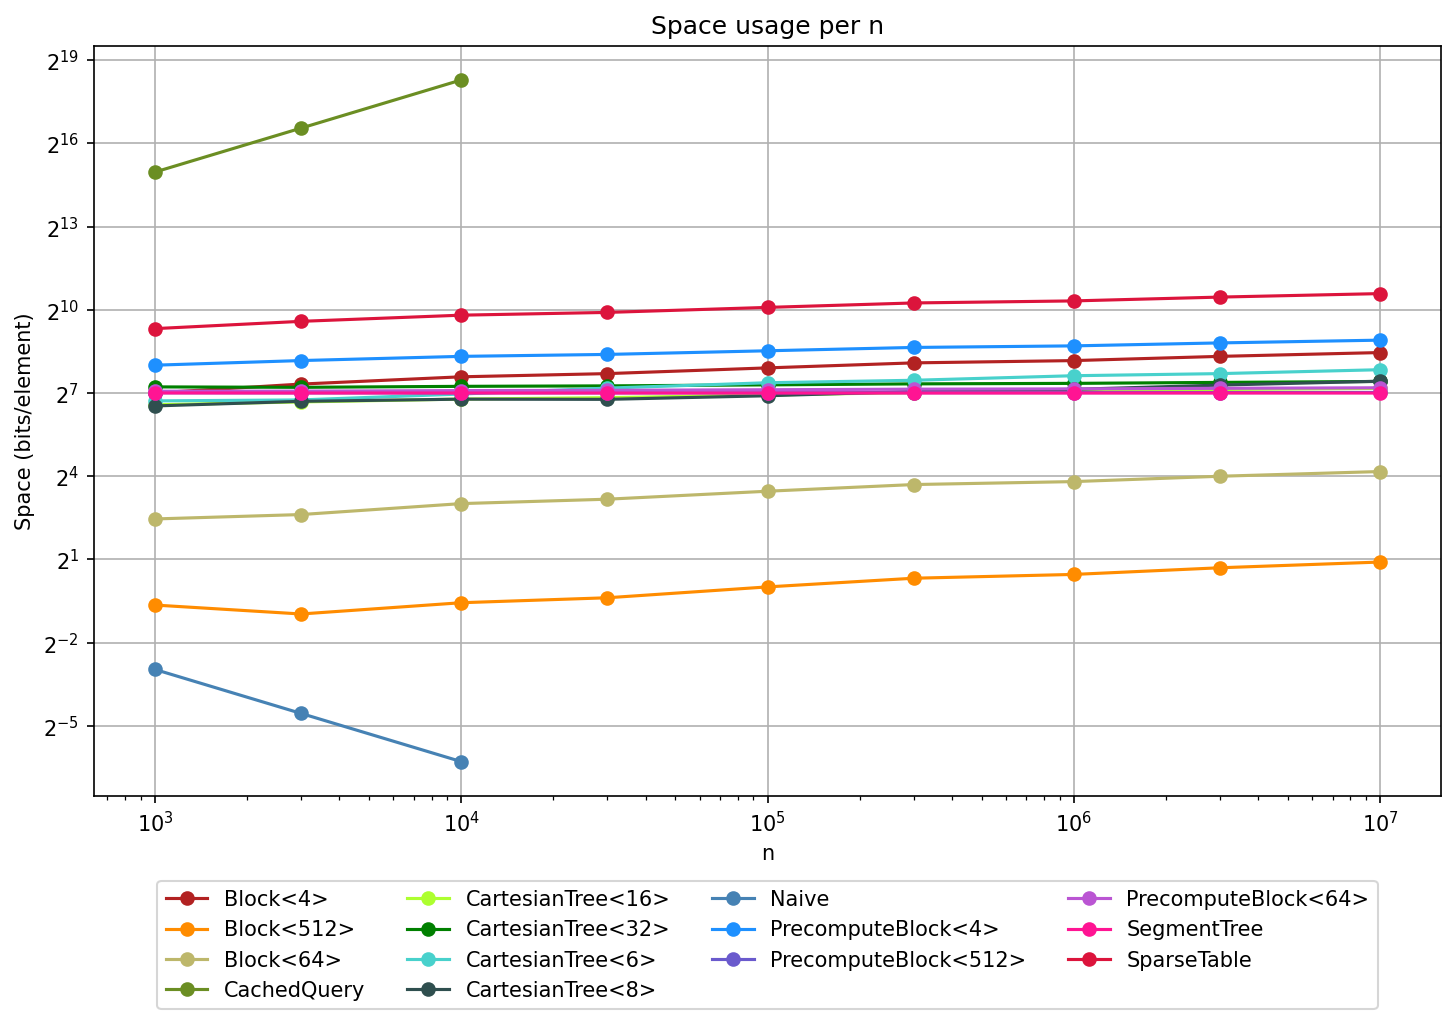
\includegraphics[width=.8\linewidth]{../plots/space.png}
	\caption{space usage}
	\label{fig:space}
\end{figure}

\subsection{Pareto Analysis}

\autoref{fig:space_time_tradeoff} shows the tradeoff between space usage and query time
for each implementation at $n=10^7$. The x-axis is logarithmic and represents the space usage in bits per element.
The y-axis is linear and represents the query time in nanoseconds. Because Naive and CachedQuery
have not been measured at this n, they are excluded from the comparison.

Block<512>, Block<64> and PrecomputeBlock<512> make up the Pareto-optimal front.
Every other implementation is dominated by one of these implementations.

In general the block implementations yield the best space-per-element usage, with 
a significant tradeoff in query time. The pre-computed block approaches are best 
in query time, closely followed by the standard sparse table. 

For a general use case, we also need to consider that pre-computed block 
implementations perform significantly worse for small n and have a high space usage.
A good overall choice would therefore be the Block<64> implementation, as it has 
slightly worse query times than, for example, the Cartesian tree approaches but 
in exchange has a significantly smaller memory footprint.


\begin{figure}[h]
	\centering
	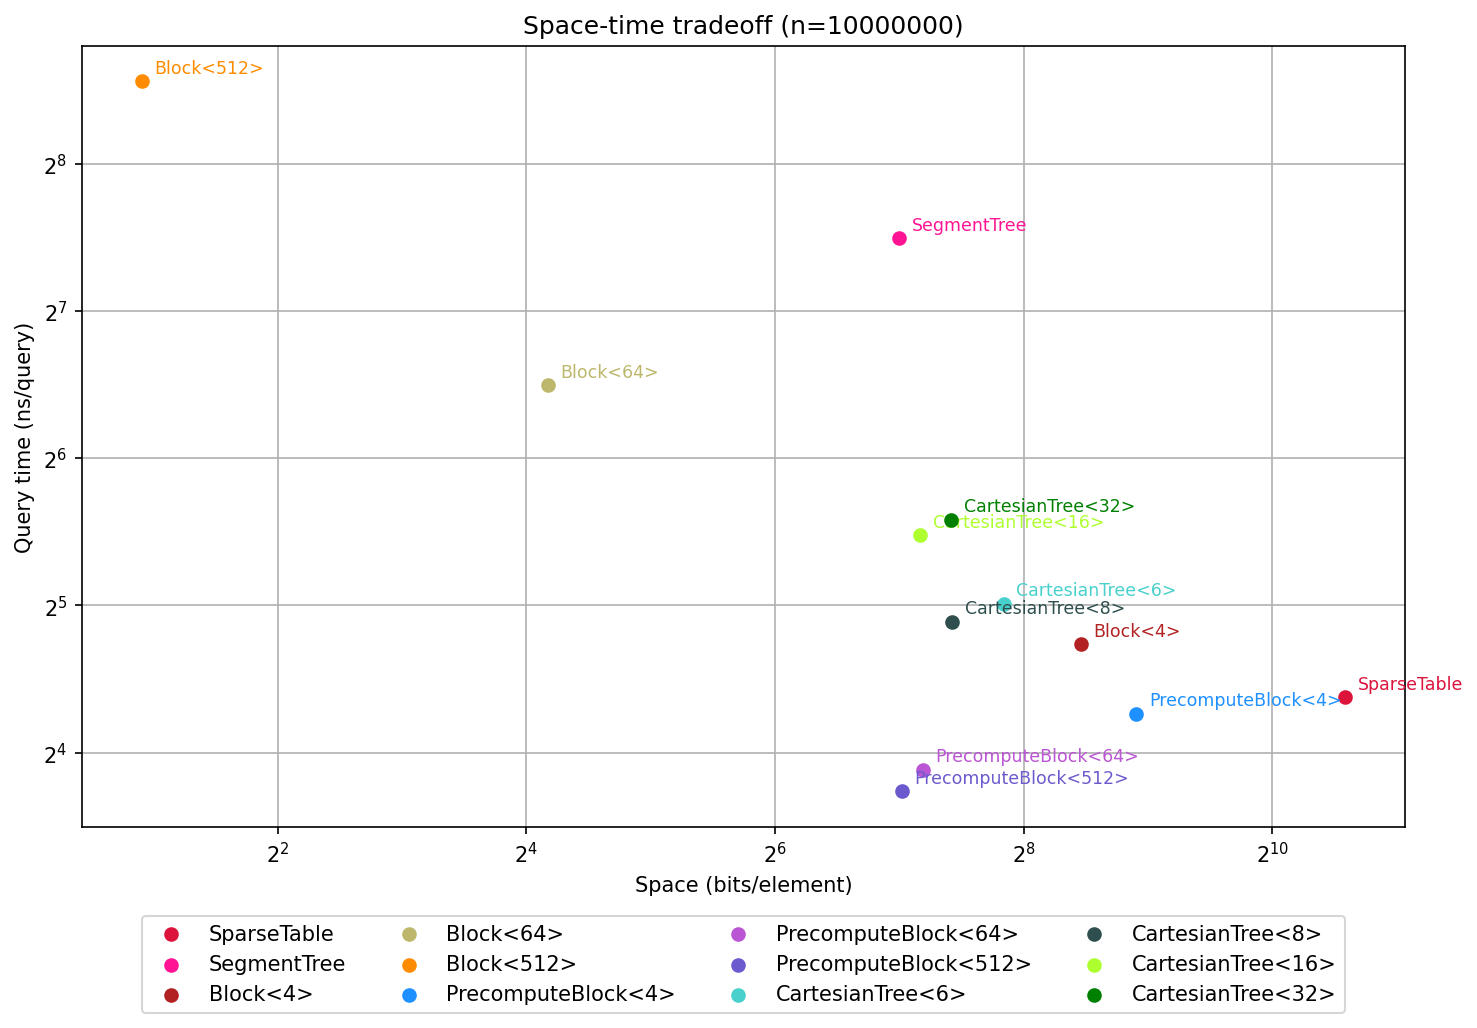
\includegraphics[width=.8\linewidth]{../plots/space_time_tradeoff.png}
	\caption{space-time trade-off}
	\label{fig:space_time_tradeoff}
\end{figure}

\subsection{Impact of Block Sizes}
\label{sec:block_sizes}

Block sizes linearly shrink the size of the underlying sparse table.
This effect is directly visible in \autoref{fig:space} for the Block<N>
implementations. The larger the block size, the smaller the sparse table and therefore the
smaller the space usage. This is a tradeoff for query time, as larger block sizes require 
an additional linear scan asymptotic to the chosen block size. 

Pre-compute block implementations trade the extra query time of blocks against
additional space for the prefix/suffix arrays. For small N, smaller blocks are better.
For larger N, all implementations have a very similar query time, making larger blocks
the better choice, as they have smaller space usage. 

For Cartesian trees, the block size has to be chosen according to the expected N.
Larger and smaller block sizes can cause higher memory usage and query time.

\subsection{Absolute Speed Considerations}

The fastest query time for $N=10^7$ is achieved by the PrecomputeBlock<512> 
implementation with 13.33ns per query. This value represents roughly 40 cycles
on the $\sim$3GHz cores of the test system and is less than a single memory access 
in DRAM with $\sim$100ns. Because N is larger than the CPU cache could possibly hold,
it is likely that the query time is dominated by parallel memory access throughput.
The used CPU has an OoO pipeline and can hold a couple of fetches in flight, while 
others are already scheduled. The latency is therefore masked by the throughput of the
memory access engine. 

To further decrease the query time, we should focus on increasing memory bandwidth, which 
could be done by working with smaller indices rather than the 64-bit values. 

\end{document}
